\chapter{Detalles de Implementación y Experimentos}\label{chapter:implementation}

Toda soluci\'on computacional, una vez concebida y dise\~nada, requiere
de una implementaci\'on pr\'actica que permita valorar la efectividad de la misma.
En el presente cap\'itulo se presentan las consideraciones esenciales y tecnolog\'ias utilizadas
para el desarrollo de un prototipo de la soluci\'on propuesta. Adem\'as, se
realiza un an\'alisis de la viabilidad del prototipo a trav\'es de la discusi\'on de los resultados
de un conjunto de experimentos.
\section{Herramientas y tecnolog\'ias utilizadas}\label{section:tools}



\subsection{Lenguaje de programaci\'on Python}

Python\footnote[1]{https://www.python.org} es un lenguaje de programaci\'on de alto nivel y de prop\'osito
general. Es interpretado, multi-paradigma, de tipado din\'amico y memoria
auto-manejada. Fue desarrollado por Guido Van Rossum en 1991 y al momento
de realizarse este trabajo est\'a disponible en su versi\'on 3.11.0.

El lenguaje presenta una sintaxis simple e intuitiva que permite su
accesibilidad por investigadores y analistas, adem\'as de programadores.
Debido al crecimiento del uso de datos en las empresas
y las facilidades que ofrece Python, el desarrollo del ecosistema profesional
del lenguaje ha sido enorme. En la actualidad cuenta con m\'ultiples bibliotecas y
paquetes cient\'ificos que proporcionan
funcionalidades dis\'imiles y son utilizados por varios campos
de la ciencia e ingenier\'ia.

En particular, existen bibliotecas especializadas en el an\'alisis de
datos, visualizaci\'on de datos, aprendizaje
de m\'aquinas tradicional y el aprendizaje de m\'aquinas sobre grafos, que
satisfacen las exigencias computacionales de la soluci\'on concebida.
A continuaci\'on se rese\~nan las bibliotecas utilizadas para
el desarrollo del prototipo.


\subsubsection{Pandas}
Pandas\footnote[2]{https://pandas.pydata.org} es una biblioteca de c\'odigo abierto orientada
a la manipulaci\'on y an\'alisis de datos. Su implementaci\'on es
r\'apida, poderosa y f\'acil de usar, lo que la ha convertido en
una herramienta muy popular entre los analistas de datos en dominios
acad\'emicos y comerciales.
Esta biblioteca es compatible con m\'ultiples formatos
de almacenamiento de datos y provee objetos para el almacenar y manipular conjuntos de datos de forma eficiente.


\subsubsection{Numpy}
Numpy\footnote[3]{https://numpy.org} es una biblioteca de c\'odigo abierto que permite crear vectores y matrices de gran
tama\~no y muchas dimensiones. Adem\'as, incluye
funciones para operar con sus matrices y vectores de una forma
c\'omoda. Internamente
utiliza el lenguaje C para la implementaci\'on de las funciones, por
lo que brinda un alto rendimiento.


\subsubsection{SciPy}
SciPy\footnote[4]{https://scipy.org} es una biblioteca de c\'odigo abierto que provee
implementaciones de algoritmos
utilizados en problemas de optimizaci\'on, integraci\'on, interpolaci\'on,
c\'alculo de valores propios, ecuaciones algebraicas, ecuaciones diferenciales y
estad\'isticas. Gracias a la utilizaci\'on de estructuras
especializadas para el c\'omputo sobre arreglos y sus implementaciones
altamente eficientes escritas en lenguajes de bajo nivel, como Fortran, C y C++,
permite resolver problemas complejos utilizando una sintaxis de alto nivel de forma r\'apida y eficiente.


\subsubsection{Scikit-Learn}
Scikit-Learn\footnote[5]{https://scikit-learn.org} es una biblioteca de aprendizaje de m\'aquinas de c\'odigo abierto.
Presenta una gran colecci\'on de modelos
para la resoluci\'on de problemas enmarcados dentro del paradigma de aprendizaje de m\'aquinas.
En la actualidad incluye modelos para problemas de clasificaci\'on, regresi\'on,
agrupamiento, reducci\'on de dimensionalidad y optimizaci\'on de modelos.

\subsubsection{Pykeen}

Pykeen\footnote[6]{https://pykeen.github.io} es una biblioteca de c\'odigo abierto dise\~nada para
entrenar y evaluar modelos de \textit{knowledge graph embedding}. Ofrece implementaciones eficientes
de m\'ultiples modelos y estrategias de entrenamiento que permiten
definir flujos de KGE en una forma sencilla.

\subsubsection{Plotly}

Plotly\footnote[7]{https://plotly.com/python/getting-started/} es una biblioteca
de c\'odigo abierto para la visualizaci\'on interactiva de datos. Esta incluye m\'as
de 40 tipos de gr\'aficos que cubren las necesidades de m\'ultiples campos del
conocimiento como la Estad\'istica, la Econom\'ia y la Geograf\'ia.


% \subsection{Google Colaboratory}
% Google Colaboratory\footnote[8]{https://colab.research.google.com} es un servicio gratuito de Google que permite escribir y ejecutar
% c\'odigo arbitrario de Python sobre recursos computacionales como GPU y TPU en
% el navegador. Esta plataforma ofrece un entorno de trabajo de Python con buenos recursos computacionales,
% bibliotecas y herramientas de aprendizaje autom\'atico pre-instaladas de forma
% gratuita.
% Basada en Jupyter Notebook brinda en su plan gratuito 13 GB de RAM, 110GB de almacenamiento (extensible mediante la utilizaci\'on de Google Drive) y
% la posibilidad de utilizar tanto CPU como GPU y TPU.


\section{Implementaci\'on del prototipo}

El prototipo implementado se compone de un conjunto de m\'odulos que se corresponden
con el dise\~no de sistema propuesto en el cap\'itulo \ref{chapter:proposal}. En las siguientes
secciones se abordan los principales desaf\'ios computacionales resueltos durante el desarrollo
de la soluci\'on.


\subsection{Conjuntos de datos y tipos de datos}
La capacidad de importar y manipular
conjuntos de datos provenientes de distintas fuentes de datos es de los aspectos m\'as importantes
del sistema. Por este motivo se utiliz\'o
la clase \texttt{DataFrame}, implementada dentro de la biblioteca Pandas, para representar
los conjuntos de datos. Esta clase implementa una gran cantidad
de operaciones de manipulaci\'on de datos y adem\'as, es compatible con distintos
formatos de almacenamiento de datos y sistemas de bases de datos relacionales.


Uno de los desaf\'ios computacionales encontrado fue la necesidad de trabajar con distintos
tipos de datos como \texttt{int}, \texttt{float}, \texttt{datetime} y \texttt{string}.
Las bibliotecas Scipy y Numpy, que son utilizadas para computar las caracter\'isticas
de los atributos,
est\'an optimizadas para la manipulaci\'on de datos num\'ericos y algunas
de sus funciones no soportan otros tipos de datos. Para solucionar este problema se utilizaron
representaciones alternativas para los tipos \texttt{datetime} y \texttt{string} que mejoran
la eficiencia computacional y espacial del sistema. Las fechas
son convertidas a enteros obteniendo la cantidad de milisegundos dentro del objeto \texttt{datetime} y los
\texttt{string} son convertidos a \texttt{int} asociando a cada cadena su tiempo de descubrimiento \texttt{t} dentro del conjunto.

Debido
a que existen existen m\'etricas distintas para las variables cuantitativas y categ\'oricas se debe considerar la clasificaci\'on
de cada tipo como variable estad\'istica. La clasificaci\'on
de los tipos \texttt{int} (cuantitativa), \texttt{float} (cuantitativa) y \texttt{string} (categ\'orica) es intuitiva. Por
otra parte, el caso de \texttt{datetime} es especial, clasific\'andose como cuantitativa si el objeto tiene
especificado la hora y categ\'orica en caso contrario. Adem\'as, para permitir el c\'omputo de m\'etricas estad\'isticas
avanzadas sobre variables categ\'oricas se decidi\'o computarlas utilizando el histograma de los datos categ\'oricos.

Por \'ultimo, existen casos en que el tipo de dato de los atributos es desconocido debido
a que el formato de almacenamiento de datos no permite almacenar metadatos sobre los atributos. Para solventar
este problema se realiza un proceso de inferencia de tipos sobre una muestra de los datos seleccionada aleatoriamente.
La inferencia se realiza mediante una serie de conversiones a los tipos soportados, registrando
en cada intento la cantidad de elementos que fallaron en la conversi\'on. El porcentaje de fallos es utilizada
como una m\'etrica para ordenar los tipos de datos de acuerdo a que tan probable sea su \'exito en la conversi\'on de los datos
originales. N\'otese que el caso del tipo \texttt{string} es especial, dado que siempre
es un tipo v\'alido, por lo que su valor de la m\'etrica se define como el complemento del m\'aximo valor obtenido por los otros tipos.
% \begin{lstlisting}[caption=Pseudoc\'odigo del c\'omputo de vectores de caracter\'isticas, label = code:build-mappings]
%     get_feature_vectors(dataset):
%         errors = dict{}
%         types = [int, float, string, datetime]
%         vectors = []

%         for attribute in dataset:
%             sample = random.sample(attribute)
%             for type in types:
%                 errors(type) = try_cast(sample, type)

%             sort(types, by=errors)
%             values = cast_until_success(attribute, types)

%             fill_missing_values(values)
%             if type in [datetime, string]:
%                 values = histogram(values)
%             feature_vector = compute_statistical_metrics(values)

%             vectors.add(feature_vector)

%         return vectors
% \end{lstlisting}


\subsection{Grafos de conocimientos}
La principal estructura de datos utilizada por el prototipo son los grafos
de conocimientos, siendo constru\'idos en las etapas de entrenamiento e inferencia
del sistema.
La implementaci\'on computacional de un grafo de conocimientos es la clase \texttt{KnowledgeGraph}. Esta
clase representa los v\'ertices del grafo mediante diccionarios que asocian las entidades a enteros, y almacena sus
aristas en una matriz, donde cada fila es una tripla (\texttt{head}, \texttt{relation}, \texttt{tail}).
Estas estructuras se construyen en dos etapas:
\begin{enumerate}
    \item \texttt{\_build\_mappings(attributes, features, encodings)} crea los mapeos de v\'ertices \texttt{categorical\_mapping} y \texttt{cuantitative\_mapping}
    que asocian los valores de las m\'etricas de los atributos a v\'ertices del grafo. Las caracter\'isticas
    categ\'oricas tienen un conjunto de posibles valores finito por tanto este mapeo es implementado
    mediante un diccionario \texttt{dict[feature:dict[value:id]]}. Las caracter\'isticas cuantitativas tienen
    un domino infinito por lo que se utiliz\'o como identificador el n\'umero del intervalo al cual pertencen en el dominio
    discretizado. Para computar el intervalo al cual pertenece un valor se realiza b\'usqueda binaria en la
    lista de puntos frontera, esto se implementa como una funci\'on an\'onima \texttt{lambda x: search(feature\_intervals, x)}
    para cada caracter\'istica. Asociando estas funciones a las caracter\'isticas se obtiene el mapeo
    cuantitativo \texttt{dict[feature:func[value,id]]}. Esta clase implementa las dos estructuras
    presentadas en el cap\'itulo \ref{chapter:ml-on-graphs} almancenando los v\'ertices, etiquetas
    y triplas de la relaci\'on \texttt{codificar} en los campos \texttt{encodings\_mapping}, \texttt{encodings} y \texttt{encodings\_triples}
    respectivamente.
    \item \texttt{\_get\_edges(attributes, mode)} itera sobre los atributos del conjunto de entrenamiento
    creando los v\'ertices asociados a estos, y devuelve el conjunto uni\'on de los conjuntos de aristas de dichos v\'ertices en una matriz.
    Al devolver el conjunto de aristas este m\'etodo tambi\'en puede ser utilizado para generar las triplas del grafo de inferencia.
\end{enumerate}

A continuaci\'on se presenta la interfaz definida para la utilizaci\'on de esta clase.
\lstset{language=Python, captionpos=b,stringstyle=\color{burntorange}}
\begin{lstlisting}[caption= Interfaz de la clase \texttt{KnowledgeGraph}, label = code:graph-generator]
    class KnowledgeGraph:

        # Nodes
        categorical_mapping : dict[feature:dict[value:id]]
        cuantitative_mapping : dict[feature:func[value,id]]
        encodings_mapping : dict[encoding:dict[value:id]]

        # Edges
        features_triples : list[[head:int, relation:int, tail:int]]
        encodings_triples : list[[head:int, relation:int, tail:int]]

        # Labels
        encodings : List[encoding]

        def __init__(self, attributes, features, encodings):
            _build_mappings(attributes, features, encodings)
            features_triples, encodings_triples = _get_edges(attributes, training=True)

        def get_inference_edges(self, attributes):
            return _get_edges(attributes, training=False)

        def _build_mappings(self, attributes, features, encoding):
            # Omitted implementation

        def _get_edges(self, attributes, training):
            # Omitted implementation
\end{lstlisting}

% \begin{lstlisting}[caption=Pseudoc\'odigo del m\'etodo \textit{\_build\_mappings}, label = code:build-mappings]

% method _build_mappings(self, attributes, features, encoding):
%     for feature in features:
%         values = attributes.get_values(feature)
%         encodings = attributes.get_values(encoding)

%         if feature.type == "categorical":
%             for value in unique(values):
%                 categorical_map(feature, value) = id()

%         if feature.type == "quantitative":
%             intervals = mdlp(values, encodings)
%             for interval in intervals:
%                 quantitative_map(feature).add(interval, id())
% \end{lstlisting}

% \begin{lstlisting}[caption= Pseudoc\'odigo del m\'etodo \textit{add\_attributes}, label = code:add-attributes]
% method add_attributes(attributes):
%     triplets = list[]

%     for attribute in attributes:
%         triplets.add((attribute.id, "encoded", attribute.encoding))

%         for feature in features:
%             value = attribute.get_value(feature)

%             if value is None:
%                 continue

%             if feature.type == "categorical":
%                 value.id = categorical_map(feature, value)

%             if feature.type == "quantitative":
%                 value.id = search(quantitative_map(feature), value)

%             triplets.add((value.id, feature.name, attribute.id))

%     return triplets


% \end{lstlisting}




\subsection{Flujos de \textit{embedding}}

En este prototipo los posibles flujos de \textit{graph embedding} est\'an definidos por los
componentes, implementados por la biblioteca Pykeen, para el entrenamiento de  estos modelos. Dentro de esta biblioteca se identificaron tres
componentes principales: modelos (\texttt{ERModel}), optimizadores (\texttt{Optimizer}) y ciclos de entrenamiento (\texttt{TrainingLoop}).
Cada uno de estos componentes tiene un conjunto de par\'ametros propios y son clases base
para m\'ultiples implementaciones dentro de Pykeen.

Para generar estos componentes se definieron clases correspondientes a cada
uno: \texttt{ERModelFactory}, \texttt{OptimizerFactory} y \texttt{TrainingLoopFactory}.
Estas consisten en un conjunto de definiciones de par\'ametros correspondientes
con los par\'ametros de las clases originales y son f\'abricas de instancias de estos componentes.
A partir de estas clases base se definen f\'abricas
de las implementaciones espec\'ificas de cada componente, las instancias de
los componentes pueden ser obtenidas
utilizando el m\'etodo \texttt{eval}.

\lstset{language=Python, captionpos=b,stringstyle=\color{burntorange}}
\begin{lstlisting}[caption= Clase f\'abrica del modelo TransE, label = code:model-factory]
class ERModelFactory:
    def __init__(self):
        self.embedding_dim = IntParam(50, 100)

    def get_model(self, triples):
        raise NotImplementedError()

class TransEFactory(ERModelFactory):
    def __init__(self):
        super().__init__()
        self.scoring_fct_norm = IntParam(1, 2)

    def eval(self, triples):
        return TransE(
            triples_factory=triples,
            embedding_dim = self.embedding_dim.eval(),
            scoring_fct_norm = self.scoring_fct_norm.eval()
        )


\end{lstlisting}


Los par\'ametros de las f\'abricas se definen mediante clases que a\~naden metadatos a los par\'ametros de
las clases de Pykeen, estos pueden ser \texttt{IntParam}, \texttt{FloatParam} y \texttt{StringParam}.
Estas clases permiten generar valores aleatorios de los par\'ametros utilizando
los metadatos con el m\'etodo \texttt{eval}. Por ejemplo, una instancia de \texttt{IntParam}
recibe dos enteros \texttt{min} y \texttt{max} en su constructor y su m\'etodo \texttt{eval} retorna
un entero aleatorio \texttt{k} tal que $\texttt{min} \leq \texttt{k} \leq \texttt{max}$.

\begin{figure}[h!]
    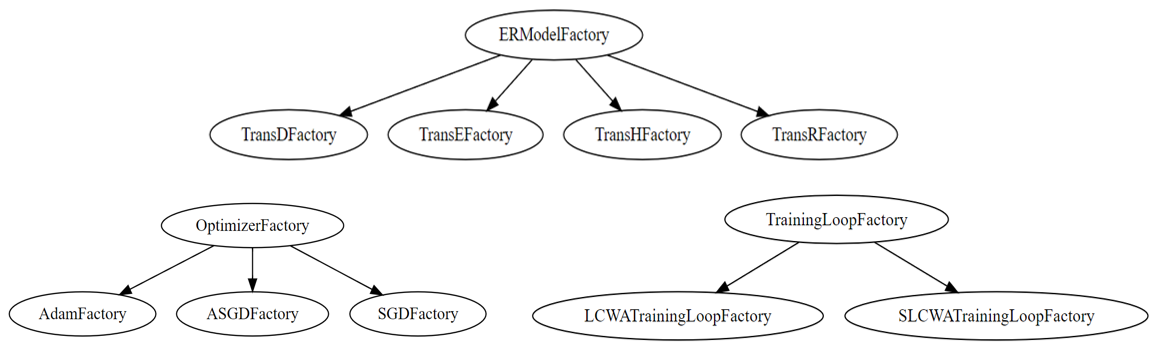
\includegraphics[width=\linewidth]{Graphics/components.png}
    \caption{Jerarqu\'ia de componentes de flujos de \textit{embedding}}
    \label{fig: emb-hierarchy}
\end{figure}

Para construir el flujo se dispone de la clase \texttt{TransductivePipelineBuilder} que utiliza introspecci\'on para
buscar implementaciones de las clases \texttt{ERModelFactory}, \texttt{OptimizerFactory} y
\texttt{TrainingLoopFactory}. Estas implementaciones son instanciadas y almacenadas
en colecciones para cada tipo de componente. Cuando un componente es necesitado se selecciona de
forma aleatoria una f\'abrica de la colecci\'on correspondiente y se invoca su m\'etodo \texttt{eval}.
Utilizando estas f\'abricas se pueden generar flujos completos de \textit{graph embedding} que respeten los par\'ametros definidos dentro de la biblioteca.

\subsection{Jerarqu\'ia de modelos}

La metaheur\'istica de universos paralelos fue implementada como
una clase abstracta que ofrece la funcionalidad de generar universos
a partir de un grafo de conocimientos y un
generador de flujos de \textit{graph embedding}.

\lstset{language=Python, captionpos=b,stringstyle=\color{burntorange}}
\begin{lstlisting}[caption= Modelo base de universos paralelos, label = code:lp-pu]
class ParallelUniverses:
    def __init__(self, knowledge_graph, pipeline_builder):
        self.knowledge_graph = knowledge_graph
        self.pipeline_builder = pipeline_builder

    def predict(self, attributes, n, ralpha, rbeta, rgamma):
        P = self.predict_proba(attributes, n, ralpha, rbeta, rgamma)
        return [argmax(v) for v in P]

    def predict_proba(self, attributes, n, ralpha, rbeta, rgamma):
        universes = self._create_parallel_universes(attributes, n, ralpha, rbeta, rgamma)
        V = self._get_voting_matrix(attributes, universes)
        P = []
        for i in range(len(X)):
            P.append(softmax(V[i,:]))
        return P

    def _get_voting_matrix(self, attributes, universes):
        raise NotImplementedError()

    def _create_parallel_universes(self, attributes, n, ralpha, rbeta, rgamma):
        # omitted implementation
\end{lstlisting}


% \lstset{language=Python, captionpos=b,stringstyle=\color{burntorange}}
% \begin{lstlisting}[caption= Modelo base de universos paralelos, label = code:lp-pu]

% class ParallelUniverses:
%     def __init__(self, knowledge_graph, pipeline_builder, n=10, ralpha, rbeta, rgamma):
%         self.knowledge_graph = knowledge_graph
%         self.pipeline_builder = pipeline_builder
%         self.n = n
%         self.ralpha = ralpha
%         self.rbeta = rbeta
%         self.rgamma = rgamma

%     def predict(self, attrs):
%         P = self.predict_proba(attrs)
%         return [argmax(v) for v in P]

%     def predict_proba(self, attrs):
%         universes = self._get_universes(attrs)
%         encodings = len(unique(self.knowledge_graph.labels))

%         V = self._get_voting_matrix(attrs, universes, encodings)

%         P = [] # probability_matrix
%         for i in range(len(X)):
%             P.append(softmax(V[i,:]))
%         return P

%     def _get_universes(self, attrs):
%         raise NotImplementedError()

%     def _get_voting_matrix(self, attrs, universes, encodings):
%         raise NotImplementedError()

%     def _create_parallel_universes(self, inference_triples, n, ralpha, rbeta, rgamma):
%         # omitted implementation

%     def _create_parallel_kg(self, inference_triples, n, ralpha, rbeta, rgamma):
%         # omitted implementation
% \end{lstlisting}
El m\'etodo \texttt{\_create\_parallel\_universes} implementa
la construcci\'on de universos paralelos descrita en el Algoritmo \ref{alg:meta-pu}. El
m\'etodo abstracto \texttt{\_get\_voting\_matrix} permite
la extensi\'on de la metaheur\'istica con diferentes implementaciones del sistema
de consenso.
A modo de ejemplo, se muestra la definici\'on del sistema de consenso basado en predicci\'on de aristas.


\lstset{language=Python, captionpos=b,stringstyle=\color{codegreen}}
\begin{lstlisting}[caption= Modelo de universos paralelos basado en predicci\'on de aristas, label = code:pl-pu]

class PuLinkPrediction(ParallelUniverses):
    def _get_voting_matrix(self, attrs, universes):
        n_encodings = len(unique(self.knowledge_graph.encodings))
        V = np.zeros((len(attrs), n_encodings))
        for model, triples in universes:
            for i, a in enumerate(attrs):
                encoding = model.predict_tail(
                    head=a.id,
                    relation="encoding"
                )
                V[i,encoding] += 1
        return V

\end{lstlisting}

% Para utilizar este sistema de consenso con algoritmos transductivos solo se necesita pasar al constructor
% de la clase un objeto \texttt{PipelineBuilder} cuyos modelos generados sean transductivos e implementar el m\'etodo
% \texttt{\_get\_universes} de la siguiente forma:

% \lstset{language=Python, captionpos=b,stringstyle=\color{codegreen}}
% \begin{lstlisting}[caption= Modelo de universos paralelos basado en predicci\'on de aristas utilizando algoritmos transductivos, label = code:trans-pl-pu]

% class TransPULinkPrediction(PULinkPrediction):
%     def _get_universes(self, attrs):
%         inference_triples = self.knowledge_graph.get_inference_edges(attrs)
%         return self._create_parallel_universes(inference_triples, self.n, self.ralpha, self.rbeta, self.rgamma)

% \end{lstlisting}

% El prototipo tambi\'en permite una futura implementaci\'on del sistema utilizando
% algoritmos inductivos:

% \lstset{language=Python, captionpos=b,stringstyle=\color{codegreen}}
% \begin{lstlisting}[caption= Modelo de universos paralelos basado en predicci\'on de aristas utilizando algoritmos inductivos, label = code:trans-pl-pu]

% class IndPULinkPrediction(PULinkPrediction):
%     def __init__(self, knowledge_graph, pipeline_builder, n, ralpha, rgamma):
%         super().__init__(knowledge_graph, pipeline_builder, n, ralpha, None, rgamma)
%         self.universes = self._create_parallel_universes(
%             attrs=None, n, ralpha, rbeta=None, rgamma)

%     def _get_universes(self, attrs):
%         return self.universes



% \end{lstlisting}

\subsection{Procesamiento en paralelo}
La velocidad de respuesta a las consultas es un aspecto
clave de todo sistema de recomendaci\'on. La metaheur\'istica de universos paralelos necesita computar
m\'ultiples \textit{embeddings} de peque\~no tama\~no al momento de realizar las
recomendaciones, lo cual puede resultar en tiempos de espera inaceptables para el usuario.
Por este motivo se decidi\'o paralelizar el proceso de entrenamiento de
los m\'ultiples modelos de \textit{embedding} generados por la metaheur\'istica.

El proceso de entrenamiento de un modelo de la biblioteca Pykeen se realiza
utilizando un objeto de la clase \texttt{TrainingLoop} asociado a este.
Adem\'as como se puede observar en el ejemplo de c\'odigo \ref{code:kge-training}
la funci\'on \texttt{train} recibe par\'ametros asociados al universo.



\lstset{language=Python, captionpos=b,stringstyle=\color{codegreen}}\label{code:kge-training}
\begin{lstlisting}[caption=Proceso de entrenamiento de los modelos de KGE, label = code:kge-trainig]
model = TransE(triples_factory=training_triples)
optimizer = Adam(params=model.get_grad_params())
training_loop = SLCWATrainingLoop(
    model=model, # takes the model as a parameter
    triples_factory = training_triples_factory,
    optimizer = optimizer
)
training_loop.train(
    triples_factory=training_triples,
    num_epochs=5, # hiperparameter
    batch_size=256 # hiperparameter
)
\end{lstlisting}

Para generar el entrenamiento de forma autom\'atica un objeto de la clase
f\'abrica \texttt{TrainingLoopFactory} genera los par\'ametros del
entrenamiento y devuelve como salida una funci\'on an\'onima que lo ejecuta.

\lstset{language=Python, captionpos=b,stringstyle=\color{codegreen}}\label{code:auto-kge-traning}
\begin{lstlisting}[caption=Generaci\'on autom\'atica de entrenamiento de KGE, label = code:auto-kge-trainig]
class SLCWAFactory(TrainingLoopFactory):
    def eval(self, triples, model, optimizer):
        loop = SLCWATrainingLoop(
            triples_factory=triples,
            model=model,
            optimizer=optimizer,
            negative_sampler_kwargs=dict(num_negs_per_pos=self.num_neg_per_pos.eval())
        )

        loop_training = lambda: loop.train(
            triples_factory=triples,
            batch_size=self.batch_size.eval(),
            clear_optimizer = self.clear_optimizer,
            num_epochs = self.num_epochs.eval(),
            use_tqdm= self.use_tqdm
        )

        return loop_training
\end{lstlisting}

Estas funciones an\'onimas son a\~nadidas a una cola
de tareas las cuales son ejecutadas por un grupo
de procesos trabajadores.

\section{Corpus}

Para poder implementar y evaluar este sistema se hace necesario contar con datos previamente clasificados.
En el contexto de la generaci\'on de configuraciones visuales esos datos ser\'ian conjuntos
de datos con su respectiva visualizaci\'on asociada. Para extraer las configuraciones gr\'aficas
estas visualizaciones deben de estar especificadas en lenguajes de visualizaci\'on de datos u otros lenguajes
de intercambio de datos como JSON \cite{pezoa2016foundations}.

A pesar de la relevancia de las funciones de recomendaci\'on dentro
de las herramientas de an\'alisis de datos, el progreso en esta l\'inea
de investigaci\'on es lastrado por la inexistencia de grandes corpus p\'ublicos.
Repositorios como WordNet \cite{wordnet1998} e IMDB Reviews \cite{maas-EtAl:2011:ACL-HLT2011} han jugado un papel importante en el desarrollo actual
del procesamiento de lenguaje natural, sin embargo, no existen repositorios similares para
los problemas enmarcados en la visualizaci\'on autom\'atica de datos.

Al momento de realizarse la presente investigaci\'on, los corpus existentes
han sido creados durante el desarrollo de sistemas basados en el aprendizaje de m\'aquinas (cap\'itulo \ref{chapter:state-of-the-art}).
Data2Vis cre\'o un corpus mediante la utilizaci\'on del sistema basado en reglas Voyager. Draco-Learn y DeepEye encargaron
la construcci\'on del corpus a un conjunto de expertos en visualizaci\'on de datos. Finalmente VizML construy\'o el primer corpus
de gran tama\~no mediante la recolecci\'on de visualizaciones publicadas en la plataforma Plotly \cite{plotly}. Debido a la gran cantidad
de datos necesitada para el entrenamiento y validaci\'on de modelos de redes neuronales se opt\'o por utilizar una versi\'on reducida
del corpus de Plotly\footnote[1]{https://kg4vis.s3.us-east-2.amazonaws.com/corpus.zip} para el desarrollo de
este trabajo.

\subsection{Preprocesamiento}\label{subsection: prepros}


El corpus de Plotly utilizado consta de 80000 visualizaciones las cuales
est\'an compuestas por un identificador y tres estructuras especificadas en JSON:
\begin{itemize}
    \item  \texttt{table\_data}: una estructura que contiene el conjunto de datos utilizado para generar la visualizaci\'on.
     \item \texttt{chart\_data}: una estructura que asocia cada cada atributo con sus configuraciones gr\'aficas.
     \item \texttt{layout}: una estructura que contiene configuraciones gr\'aficas avanzadas como los m\'argenes y rangos.
\end{itemize}

Se procedi\'o a extraer de \texttt{table\_data} los conjuntos de datos, comprobando que estos no estuviesen vac\'ios, para ser
 procesados por
el m\'odulo de extracci\'on de caracter\'isticas. Una vez obtenido un corpus de vectores de caracter\'isticas estos fueron asociados con sus correspondientes
configuraciones gr\'aficas (tipo de marca y eje) extra\'idas de la estructura \texttt{chart\_data}. Luego se comprob\'o
que cada atributo estuviera asociado a una y solo una opci\'on por cada configuraci\'on gr\'afica.

Al descartar aquellas visualizaciones
que incumpl\'ian las restricciones de integridad se obtuvo un nuevo corpus de 60206 visualizaciones y 169178 atributos con un promedio de
2.8 atributos por visualizaci\'on.
%\vspace{0.4cm}

\begin{table}[H]
    \centering
    \begin{tabular}{ |c|c|c|}
        \hline
        \bf Marca & \bf Eje x & \bf Eje y\\
        \hline
        barra & 12299 & 245454 \\
        caja & 822 & 8273\\
        mapa de calor & 25  & 21\\
        histograma & 3157 & 330 \\
        l\'inea & 16976 & 40280  \\
        puntos & 23893 & 38557 \\
        \hline


    \end{tabular}
    \caption{Distribuci\'on de atributos respecto al tipo de marca y eje}
    \label{tab:corpus-dist}
\end{table}


% \begin{table}[H]
%     \centering
%     \begin{tabular}{ |c|c|c|c|}
%         \hline
%          & x & y & total\\
%         \hline
%         barra & 12299 & 24545 & 36844 \\
%         \hline
%         caja & 822 & 8273 & 9095\\
%         \hline
%         mapa de calor & 25  & 21 & 46 \\
%         \hline
%         histograma & 3157 & 330 & 3487\\
%         \hline
%         l\'inea & 16976 & 40280 & 57256 \\
%         \hline
%         puntos & 23893 & 38557 & 62450\\
%         \hline
%         total & 57172 & 112006 & 169178\\
%         \hline

%     \end{tabular}
%     \caption{Distribuci\'on de atributos respecto al tipo de marca y eje}
%     \label{tab:corpus-dist}
% \end{table}


Tomando en consideraci\'on la distribuci\'on mostrada en la Tabla \ref{tab:corpus-dist} se decidi\'o utilizar
aquellas visualizaciones cuyo tipo de marca sea barra, l\'inea o punto.
Finalmente, se muestrearon los conjuntos de datos de forma estratificada con respecto al tipo de marca y seleccionando un atributo
por eje en cada conjunto de datos,
cre\'andose un corpus de 15000 conjuntos de datos.
%\vspace{0.4cm}


\section{Experimentaci\'on}

Para comprobar la viabilidad de la soluci\'on computacional propuesta,
se implement\'o un prototipo como primera aproximaci\'on, sobre cuya
especificaci\'on se concibi\'o y ejecut\'o un conjunto de experimentos.
A continuaci\'on se describir\'a el dise\~no de los experimentos, as\'i
como se presentar\'an y evaluar\'an sus resultados.

\subsection{Escenario de prueba}


\begin{itemize}
    \item Corpus: Se utiliz\'o el corpus cuya construcci\'on se abord\'o en la
    secci\'on \ref{subsection: prepros}. Este fue dividido de forma estratificada en dos conjuntos disjuntos, uno de entrenamiento
    y otro de evaluaci\'on, con una proporci\'on 4 a 1.

    \item Equipo: Se utiliz\'o una computadora port\'atil con un procesador Intel(R) Core(TM) i5-9300H CPU @2.40GHz x 4, 16GB de memoria RAM y
    sistema operativo Debian 11.5 Bullseye
\end{itemize}

\subsection{Dise\~no y resultados de los experimentos}
    Se dise\~naron un total de 4 experimentos que permiten evaluar
    los modelos espec\'ificos propuestos y el sistema de recomendaci\'on en
    general.

    \subsubsection{Experimento 1: Evaluaci\'on de los modelos de universos paralelos}

    El objetivo del experimento es comprobar la efectividad de los modelos
    de universos paralelos PuLinkPrediction (PuLP) y PuNodeClassification (PuNC)
    en las dos tareas de clasificaci\'on existentes
    en el corpus: \begin{itemize}
        \item Dado un atributo clasificarlo de acuerdo a su tipo de marca en \texttt{barra}, \texttt{l\'inea} o \texttt{punto}.
        \item Dado un atributo clasificarlo de acuerdo a su tipo de eje en \texttt{x} o \texttt{y}.
    \end{itemize}
    Este experimento se divide en dos fases por cada tarea de clasificaci\'on:
    \begin{enumerate}
        \item Inicializaci\'on de la instancia del modelo con par\'ametros seleccionados manualmente y construcci\'on del
        grafo de entrenamiento.
        \item Predicci\'on de las clases para cada atributo.
    \end{enumerate}

    Los resultados obtenidos fueron evaluados utilizando la precisi\'on de los modelos, esta
    se calcula dividiendo
    el n\'umero de predicciones correctas entre el total de predicciones realizadas. Los valores
    de esta m\'etrica fueron comparados utilizando como referencia los
    resultados publicados por Hu y col. \cite{hu2019vizml}.

    \begin{table}[H]
        \centering
        \begin{tabular}{ |c|c|c|c|}
            \hline
            \bf Modelo  & \bf P(marca) & \bf P(eje)\\
            \hline
            PuNC  & 0.583& 0.708\\
            PuLP  & 0.627 & 0.754\\
            \hline
        
            VizML  & \bf 0.678 & \bf 0.831\\
            \hline
            NB  & 0.411 & 0.700 \\
            KNN  & 0.519 & 0.656\\
            LR  & 0.526 & 0.791\\
            RF  &  0.601& 0.830\\
            \hline

        \end{tabular}
        \caption{Comparativa de los resultados obtenidos por los modelos de universos paralelos y otros modelos del estado del arte.
        NB(Naive Bayes), KNN(K-Nearest Neighbors), LR(Logistic Regression), RF(Random Forest).
        }
    \end{table}

    Entre los modelos propuestos el que mejor precisi\'on obtuvo en ambas tareas fue el modelo PuLP. El modelo
    implementado por VizML, basado en redes neuronales, fue el de mejores resultados obteniendo un 5\% y 8\% m\'as de precisi\'on
    que PuLP en la clasificaci\'on del tipo de marca y eje respectivamente.
    El proceso de evaluaci\'on de los modelos dur\'o un promedio de
    12 horas y 39 minutos, con un promedio de 15.18 segundos por atributos. Estos
    resultados confirman la validez de los modelos implementados para la resoluci\'on de las tareas
    de selecci\'on de configuraciones gr\'aficas propuestas. Sin embargo, demuestran la imposibilidad
    de utilizarlos en un sistema de recomendaci\'on de configuraciones gr\'aficas que genere las
    recomendaciones de forma din\'amica, siendo necesaria la experimentaci\'on con estrategias
    de prec\'omputo que permitan su utilizaci\'on.

    \subsubsection{Experimento 2: Evaluaci\'on de los modelos de universos paralelos utilizando lotes}

    Debido al alto tiempo necesitado para realizar predicciones procesando
    los atributos uno por uno, se opt\'o por realizar este proceso
    en lotes de atributos. El objetivo de este experimento es
    evaluar el efecto del esquema de predicci\'on en lotes sobre la precisi\'on
    de los modelos, comparando los resultados con los del experimento anterior.

    \begin{table}[H]
        \centering
        \begin{tabular}{ |c|c|c|c|}
            \hline
            \bf N &  \bf P(marca) & \bf P(eje)& \bf Tiempo(s)\\
            \hline
            1 & 0.627 & 0.754 & 15.18 \\
            10 & 0.627&  0.754&  15.23\\
            20 & 0.623 & 0.747 & 16.04\\
            30 & 0.615  & 0.742 & 17.38\\
            40 & 0.586 & 0.718 & 19.45\\
            50 & 0.572 & 0.679 & 22.52\\
            \hline

        \end{tabular}
        \caption{Resultados obtenidos por el modelo PuLinkPrediction utilizando un
        esquema de predicci\'on por lotes. El tiempo se expresa en segundos por lote procesado.}
        \label{tab:lotes}
    \end{table}

    Como se puede observar en la tabla \ref{tab:lotes} al incrementar el tama\~no del lote
    se produce un decremento en la precisi\'on del modelo, sin embargo, esta p\'erdida es marginal
    para tama\~nos de lote $N \leq 30$. Por tanto, se consider\'o viable realizar
    la evaluaci\'on en lotes, durante una fase de prec\'omputo, para mejorar los tiempos de respuesta del sistema de recomendaci\'on.


    \subsubsection{Experimento 3: Evaluaci\'on del sistema de recomendaci\'on de configuraciones gr\'aficas}

    A partir del experimento anterior se decidi\'o realizar el c\'omputo de las recomendaciones
    en una etapa de preprocesamiento luego de ser recibido el conjunto de datos.
    El objetivo del experimento es evaluar las capacidades del sistema
    de recomendaci\'on de configuraciones gr\'aficas implementado
     de acuerdo a los criterios de: \begin{itemize}
    \item Efectividad de las recomendaciones realizadas.
    \item Tiempo de preprocesamiento de las consultas.
    \end{itemize}
Este experimento se realiza en dos fases:
\begin{enumerate}
    \item Inicializaci\'on del sistema mediante la selecci\'on manual de par\'ametros y entrenamiento
    de los modelos.
    \item Predicci\'on de una lista de $k$ visualizaciones para cada conjunto de datos.
\end{enumerate}

    Las predicciones obtenidas fueron evaluadas empleando la medida de proporci\'on
    de aciertos Hits@k. Esta es calculada como la fracci\'on de los conjuntos de datos cuya configuraci\'on gr\'afica
    esperada fue inclu\'ida en la lista de $k$ visualizaciones recomendadas. Adem\'as, se midi\'o
    el tiempo transcurrido durante la fase de predicci\'on y este fue promediado con la cantidad de conjuntos de datos
    procesados.


 \begin{table}[H]
        \centering
        \begin{tabular}{ |c|c|c|c|}
            \hline
            \bf Modelo & \bf Hits@1 & \bf Hits@3 & \bf Hits@5\\
            \hline
            PuLP & 0.380&  0.548& 0.662\\
            PuNC &  0.280& 0.421& 0.503\\
            Random &  0.027 & 0.083 & 0.138\\
            \hline
        \end{tabular}
        \caption{Resultados obtenidos por los modelos de universos paralelos en la recomendaci\'on de visualizaciones.}
    \end{table}

    Los modelos desarrollados obtuvieron mucho mejores resultados que los obtenidos por la recomendaci\'on aleatoria
    de visualizaciones, siendo PuLP el mejor modelo logrando recomendar la visualizaci\'on
    buscada en su top 5 un 66\% de las veces.
    Durante este experimento se procesaron en lotes de 30 un total de 6000 atributos en un tiempo de 30 minutos y 24 segundos, con un promedio de 0.608 segundos
    por atributo. Estos resultados confirman la capacidad del sistema de recomendaci\'on de sugerir las visualizaciones
    correctas con tiempos de prec\'omputo aceptables mediante la utilizaci\'on 
    de un esquema de evaluaci\'on por lotes.

    \subsubsection{Experimento 4: An\'alisis exploratorio de los jugadores m\'as valiosos de TransferMarket}

    Este experimento fue dise\~nado para simular la utilizaci\'on del sistema en un caso
    real. Para ello, se obtuvo un conjunto de datos\footnote[1]{https://www.kaggle.com/datasets/machinemind/transfermarket-mvps-dec2019} de la plataforma Kaggle que recopila
    los datos de los jugadores de f\'utbol m\'as valiosos en diciembre del a\~no 2019, seg\'un la p\'agina especializada TransferMarket.

    Este conjunto de datos cuenta con un total de 7 columnas: Rango, Nombre, Edad, Posici\'on, Pa\'is, Club y Valor.
    El n\'umero de columnas fue aumentado utilizando funciones de agregaci\'on: \begin{itemize}
        \item Las variables categ\'oricas Nombre, Posici\'on, Pa\'is y Club fueron agregadas mediante
        la funci\'on \texttt{COUNT}, utilizando el resto de variables categ\'oricas para realizar la operaci\'on \texttt{GROUP BY}.
        \item Las variables cuantitativas Rango, Edad y Valor fueron agregadas mediante las funciones \texttt{AVG}, \texttt{MAX}, \texttt{MIN} y \texttt{SUM}
        utilizando las variables categ\'oricas para realizar la operaci\'on \texttt{GROUP BY}.

    \end{itemize}

    Al finalizar el proceso de agregaci\'on se obtuvieron un total de 48 columnas. Estas
    fueron procesadas en dos lotes, de 30 y 18 columnas cada uno, en un tiempo de 56 segundos por el sistema de
    recomendaci\'on basado en el modelo PuLinkPrediction. Luego se procedi\'o a realizar
    un conjunto de consultas que son especificadas por dos atributos y, opcionalmente,
    las funciones de agregaci\'on aplicadas sobre los atributos. La respuesta a las consultas se produce de forma instant\'anea
    empleando las puntuaciones previamente computadas obteni\'endose una lista de gr\'aficos recomendados para cada una (Figura \ref{fig: results}).


    \begin{figure}[h!]
        \centering
        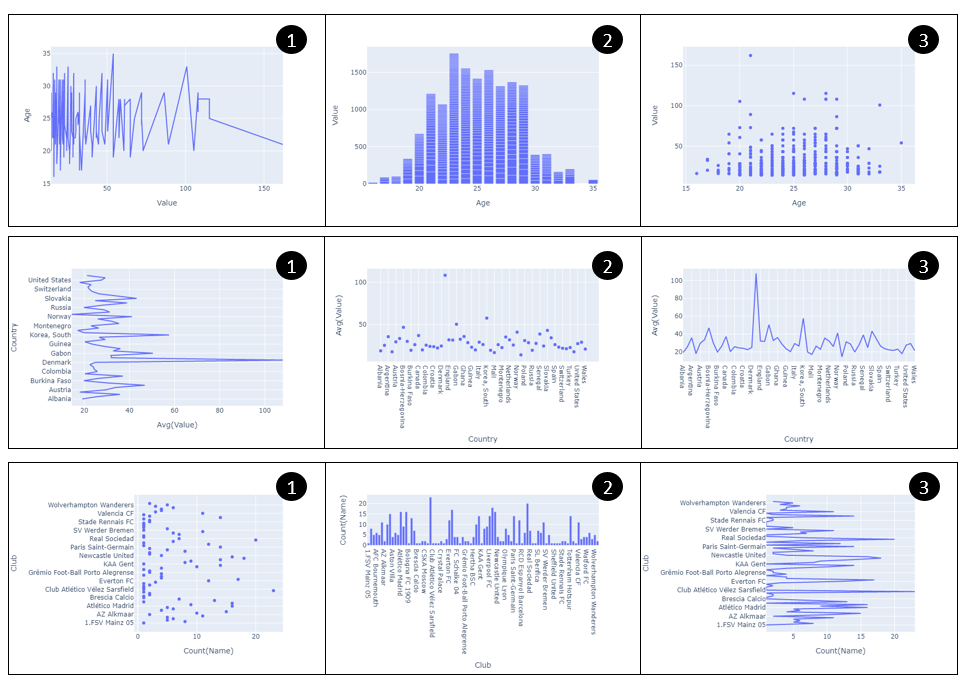
\includegraphics[width=120mm]{Graphics/results.png}
        \caption{Salida del sistema para las consultas (Edad, Valor),\\
        (Pa\'is, \texttt{AVG}(Valor \texttt{GROUP BY} Pa\'is)) y (Club, \texttt{COUNT}(Name \texttt{GROUP BY} Club)).\\ Se muestra solamente el top 3 de las recomendaciones.}
        \label{fig: results}
    \end{figure}

    \section{Discusi\'on}

    A partir de los experimentos realizados se puede observar que los modelos dise\~nados no obtuvieron
    una precisi\'on muy alta. Sin embargo, sus resultados han sido no muy distintos a los mostrados por otros modelos
    del estado del arte. El modelo basado en predicci\'on de aristas obtuvo de forma sistem\'atica
    mejores resultados que el modelo basado en clasificaci\'on de v\'ertices. Se comprob\'o que estos modelos no pueden ser utilizados para generar
    visualizaciones de forma din\'amica, sino que deben ser precomputadas utilizando una evaluaci\'on
    por lotes.

    Utilizando estos modelos se desarroll\'o un sistema de recomendaci\'on de configuraciones gr\'aficas,
    que propuso la visualizaci\'on buscada 6 de cada 10 veces en su top 5, para los conjuntos de datos
    del corpus de entrenamiento. Finalmente, se dise\~n\'o un experimento para simular la utilizaci\'on
    de este sistema en un caso real, obteni\'endose un  tiempo aceptable de preprocesamiento y respuesta a las consultas.

    Todas las instancias de modelos utilizadas en estos experimentos fueron
    inicializadas con los mismos par\'ametros $|\Delta| = 15$, $\alpha \in (7,15)$, $\beta \in (100, 200)$ y $\gamma \in (200, 300)$.
    Estos fueron escogidos de forma manual, mediante un proceso de prueba y error, para mejorar
    la precisi\'on de los modelos. Todos estos par\'ametros intervienen
    directamente en el rendimiento del modelo al especificar
    la cantidad de universos paralelos generados y su complejidad. Debido a
    esto, la optimizaci\'on de los par\'ametros no puede estar dirigida a mejorar 
    \'unicamente la precisi\'on, sino a obtener el mejor balance entre el rendimiento del modelo y sus resultados.

    Los algoritmos de \textit{knowledge graph embedding} seleccionados tambi\'en deben ser considerados
    en el estudio de los resultados obtenidos y en trabajos futuros. En las condiciones del problema a resolver, donde
    no se puede emplear mucho tiempo en el entrenamiento de los modelos, la rapidez de convergencia
    de los algoritmos utilizados pudiese ser un factor que permita mejorar los modelos concebidos.